\documentclass[11pt]{article}
\usepackage[a4paper,margin=1.9cm]{geometry}
\usepackage[T1]{fontenc}
\usepackage{textcomp}
\usepackage{amsmath,amssymb}
\usepackage{enumitem}
\usepackage{tikz}
\usetikzlibrary{calc,arrows.meta,patterns,decorations.pathmorphing}
\usepackage{xcolor}
\usepackage{multicol}
\usepackage{parskip}
\usepackage{lmodern}
\renewcommand{\familydefault}{\sfdefault}

\definecolor{unalblue}{RGB}{31,73,124}
\definecolor{solgreen}{RGB}{20,110,70}

\newlist{opciones}{enumerate}{1}
\setlist[opciones]{label=(\alph*),itemsep=1pt,topsep=2pt,leftmargin=1.8em,font=\normalfont}

\newcommand{\vect}[2]{\begin{pmatrix}#1\\#2\end{pmatrix}}
\newcommand{\vectiii}[3]{\begin{pmatrix}#1\\#2\\#3\end{pmatrix}}
\newcommand{\sol}{\medskip\noindent\textbf{\textcolor{solgreen}{Soluci\'on.}}\ }

\newcommand{\examheader}{%
  \noindent
  \begin{minipage}[t]{0.62\linewidth}
    {\bfseries\large C\'alculo en Varias Variables (1000006)}\\
    {\small Primer examen parcial}\\
    {\small Semestre 01-2013, 8 de abril de 2013}\\
    {\small Universidad Nacional de Colombia, Sede Medell\'in, Escuela de Matem\'aticas.}
  \end{minipage}%
  \hfill
  \begin{minipage}[t]{0.33\linewidth}
    \raggedleft\small
    Nombre y carnet: \rule{2.5cm}{0.4pt}\\[4pt]
    Profesor y grupo: \rule{2.5cm}{0.4pt}
  \end{minipage}\\[4pt]
  \rule{\linewidth}{0.6pt}
}
\newcommand{\examfooter}{%
  \vfill
  \rule{\linewidth}{0.4pt}\\[1pt]
  {\scriptsize\textit{Transcripci\'on digital con soluci\'on --- MathUNAL}\hfill\textcolor{unalblue}{\textbf{\thepage}}}
}
\pagestyle{empty}

\begin{document}

\examheader

\textbf{Duraci\'on:} 1 hora y 50 minutos.

\textbf{Instrucciones.} No est\'a permitido el uso de calculadora ni de cualquier otro tipo de aparato electr\'onico, incluyendo tel\'efonos m\'oviles, los cuales deben permanecer apagados durante el tiempo de duraci\'on del examen. Tampoco est\'a permitido hacer preguntas a las personas encargadas de la vigilancia.

\medskip
El examen consta de 4 puntos distribuidos en 4 p\'aginas.

\bigskip
\noindent\textbf{1.} (25\,\%)
\begin{opciones}
  \item[a.] (12\,\%) Encuentre y dibuje el dominio de la funci\'on
  $$f(x,y) = \sqrt{4-x^2-y^2} + \ln(x^2+y^2-1).$$
  \item[b.] (13\,\%) Determine si existe
  $$\lim_{(x,y)\to(0,0)} \frac{2\sin(x^2+y^2)+x^4}{x^2+y^2}.$$
\end{opciones}

\sol \textbf{a)} Necesitamos $4-x^2-y^2\geq 0$ (para la ra\'iz) y $x^2+y^2-1>0$ (para el logaritmo), es decir
$$1 < x^2+y^2 \leq 4.$$
El dominio es el anillo circular centrado en el origen, sin incluir la circunferencia interior de radio $1$ pero incluyendo la circunferencia exterior de radio $2$:

\begin{center}
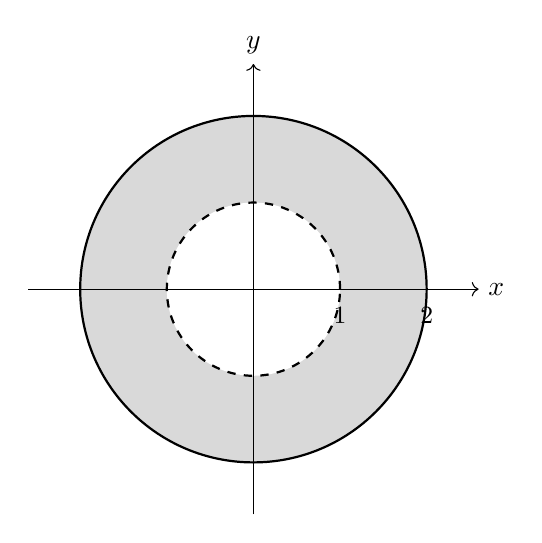
\begin{tikzpicture}[scale=1.1]
  \fill[gray!30] (0,0) circle (2);
  \fill[white] (0,0) circle (1);
  \draw[thick] (0,0) circle (2);
  \draw[thick,dashed] (0,0) circle (1);
  \draw[->] (-2.6,0) -- (2.6,0) node[right]{$x$};
  \draw[->] (0,-2.6) -- (0,2.6) node[above]{$y$};
  \node[below] at (1,-0.1) {\small $1$};
  \node[below] at (2,-0.1) {\small $2$};
\end{tikzpicture}
\end{center}

\textbf{b)} Sea $r^2=x^2+y^2$. Usando el l\'imite notable $\dfrac{\sin(r^2)}{r^2}\to 1$ cuando $r\to 0$:
$$\frac{2\sin(x^2+y^2)}{x^2+y^2} \xrightarrow[(x,y)\to(0,0)]{} 2.$$
Adem\'as, como $x^4\leq (x^2+y^2)^2=r^4$,
$$0 \leq \frac{x^4}{x^2+y^2} \leq r^2 \xrightarrow[(x,y)\to(0,0)]{} 0.$$
Por lo tanto el l\'imite existe y vale
$$\lim_{(x,y)\to(0,0)} \frac{2\sin(x^2+y^2)+x^4}{x^2+y^2} = 2+0 = 2.$$

\newpage
\examheader
\vspace{2pt}

\noindent\textbf{2.} (25\,\%) Sea $f:\mathbb{R}^2 \longrightarrow \mathbb{R}$ la funci\'on definida por
$$
f(x,y)=
\begin{cases}
\dfrac{x^3-2y^3}{x^2+y^2}, & (x,y)\neq (0,0),\\[6pt]
0, & (x,y)=(0,0).
\end{cases}
$$
\begin{opciones}
  \item[a.] (12\,\%) Encuentre las derivadas parciales $f_x(0,0)$ y $f_y(0,0)$.
  \item[b.] (13\,\%) Es $f$ diferenciable en $(0,0)$?
\end{opciones}

\sol \textbf{a)} Por definici\'on,
$$f_x(0,0) = \lim_{h\to 0} \frac{f(h,0)-f(0,0)}{h} = \lim_{h\to 0} \frac{h^3/h^2}{h} = \lim_{h\to 0} 1 = 1,$$
$$f_y(0,0) = \lim_{h\to 0} \frac{f(0,h)-f(0,0)}{h} = \lim_{h\to 0} \frac{-2h^3/h^2}{h} = \lim_{h\to 0} (-2) = -2.$$

\textbf{b)} Estudiamos el error respecto al plano candidato $L(x,y)=x-2y$:
$$E(x,y) = \frac{f(x,y)-x+2y}{\sqrt{x^2+y^2}} = \frac{\dfrac{x^3-2y^3}{x^2+y^2}-x+2y}{\sqrt{x^2+y^2}} = \frac{x^3-2y^3-x(x^2+y^2)+2y(x^2+y^2)}{(x^2+y^2)^{3/2}}.$$
Expandiendo el numerador:
$$x^3-2y^3-x^3-xy^2+2x^2y+2y^3 = 2x^2y - xy^2 = xy(2x-y).$$
As\'i,
$$E(x,y) = \frac{xy(2x-y)}{(x^2+y^2)^{3/2}}.$$
Tomando la trayectoria $x=y$:
$$E(y,y) = \frac{y\cdot y\,(2y-y)}{(2y^2)^{3/2}} = \frac{y^3}{2\sqrt2\,|y|^3} = \frac{\operatorname{sgn}(y)}{2\sqrt2},$$
que no tiende a $0$ cuando $y\to 0$ (vale $\pm\frac{1}{2\sqrt2}$ seg\'un el signo de $y$). Por lo tanto
$$\lim_{(x,y)\to(0,0)} E(x,y) \neq 0,$$
y $f$ \textbf{no} es diferenciable en $(0,0)$.

\bigskip
\noindent\textbf{3.} (25\,\%)
\begin{opciones}
  \item[a.] (12\,\%) En cu\'al direcci\'on la funci\'on $f(x,y)=1-x^2-y^2$ crece m\'as r\'apidamente en $(1,1)$? Encuentre el valor de la m\'axima raz\'on de cambio de $f$ en $(1,1)$.
  \item[b.] (13\,\%) Encuentre los puntos en el hiperboloide $x^2+4y^2-z^2=4$ donde el plano tangente es paralelo al plano $2x+2y+z=5$.
\end{opciones}

\sol \textbf{a)} $\nabla f(x,y)=(-2x,-2y)$, luego $\nabla f(1,1)=(-2,-2)$. La direcci\'on de mayor crecimiento es la del gradiente, normalizada:
$$\hat u = \frac{(-2,-2)}{\|(-2,-2)\|} = \left(-\frac{1}{\sqrt2},\,-\frac{1}{\sqrt2}\right),$$
y la m\'axima raz\'on de cambio es
$$\|\nabla f(1,1)\| = \sqrt{(-2)^2+(-2)^2} = 2\sqrt2.$$

\textbf{b)} Sea $G(x,y,z)=x^2+4y^2-z^2$ (superficie de nivel $G=4$). El gradiente $\nabla G=(2x,8y,-2z)$ debe ser paralelo al vector normal del plano dado, $(2,2,1)$:
$$(2x,8y,-2z) = t(2,2,1) \implies x=t,\quad y=\frac{t}{4},\quad z=-\frac{t}{2}.$$
Sustituyendo en la ecuaci\'on del hiperboloide:
$$t^2 + 4\left(\frac{t}{4}\right)^2 - \left(-\frac{t}{2}\right)^2 = 4 \;\Longrightarrow\; t^2+\frac{t^2}{4}-\frac{t^2}{4} = 4 \;\Longrightarrow\; t^2=4 \;\Longrightarrow\; t=\pm 2.$$
Para $t=2$: el punto es $\left(2,\ \tfrac12,\ -1\right)$. Para $t=-2$: el punto es $\left(-2,\ -\tfrac12,\ 1\right)$.

\newpage
\examheader
\vspace{2pt}

\noindent\textbf{4.} (25\,\%) Sea $z=f(x,y)$ una funci\'on de clase $C^2$ y sean $x=r\cos\theta$, y $y=r\operatorname{sen}\theta$. Pruebe que
$$z_{rr} = f_{xx}\cos^2\theta + 2f_{xy}\cos\theta\operatorname{sen}\theta + f_{yy}\operatorname{sen}^2\theta.$$

\sol Por la regla de la cadena,
$$z_r = f_x\,x_r + f_y\,y_r = f_x\cos\theta + f_y\operatorname{sen}\theta.$$
Derivando de nuevo respecto de $r$ (recordando que $f_x$ y $f_y$ dependen de $x,y$, que a su vez dependen de $r$):
$$z_{rr} = \frac{\partial}{\partial r}(f_x)\cos\theta + \frac{\partial}{\partial r}(f_y)\operatorname{sen}\theta.$$
Como
$$\frac{\partial}{\partial r}(f_x) = f_{xx}\,x_r + f_{xy}\,y_r = f_{xx}\cos\theta + f_{xy}\operatorname{sen}\theta,$$
$$\frac{\partial}{\partial r}(f_y) = f_{yx}\,x_r + f_{yy}\,y_r = f_{xy}\cos\theta + f_{yy}\operatorname{sen}\theta \quad (\text{pues } f_{xy}=f_{yx} \text{ al ser } f\in C^2),$$
sustituyendo:
$$z_{rr} = \big(f_{xx}\cos\theta + f_{xy}\operatorname{sen}\theta\big)\cos\theta + \big(f_{xy}\cos\theta + f_{yy}\operatorname{sen}\theta\big)\operatorname{sen}\theta$$
$$= f_{xx}\cos^2\theta + f_{xy}\cos\theta\operatorname{sen}\theta + f_{xy}\cos\theta\operatorname{sen}\theta + f_{yy}\operatorname{sen}^2\theta$$
$$= f_{xx}\cos^2\theta + 2f_{xy}\cos\theta\operatorname{sen}\theta + f_{yy}\operatorname{sen}^2\theta. \qquad \blacksquare$$

\vfill
\examfooter

\end{document}
